\documentclass[conference]{IEEEtran}

% Packages
\usepackage{cite}
\usepackage{amsmath,amssymb,amsfonts}
\usepackage{algorithmic}
\usepackage{algorithm}
\usepackage{graphicx}
\usepackage{textcomp}
\usepackage{xcolor}
\usepackage{booktabs} % For professional quality tables
\usepackage{url}
\usepackage{tikz} % For drawing flowcharts
\usetikzlibrary{shapes.geometric, arrows, positioning, fit, calc}

% Define BibTeX style
\def\BibTeX{{\rm B\kern-.05em{\sc i\kern-.025em b}\kern-.08em
    T\kern-.1667em\lower.7ex\hbox{E}\kern-.125emX}}

\begin{document}

\title{A Smart Campus Framework for Personalized Information Delivery Using Intelligent Digital Billboards}
\author{
    \IEEEauthorblockN{Dr. Newbegin Luke, Dr. Chanti S, Dr. Surabhi Saxena}
    \IEEEauthorblockA{\textit{Department of Computer Science} \\
    \textit{Christ (Deemed to be University)}\\
    Bengaluru, India \\
    \{newbegin.luke, chanti.s, surabhi.saxena\}@christuniversity.in}
    \and
    \IEEEauthorblockN{Sachin Yadav and Surya Vamshi S}
    \IEEEauthorblockA{\textit{Department of Computer Science} \\
    \textit{Christ (Deemed to be University)}\\
    Bengaluru, India \\
    \{sachin.yadav, surya.s\}@bcah.christuniversity.in}
}


\maketitle

\begin{abstract}
This paper proposes a smart campus system designed to improve how students receive information. By using digital billboards equipped with cameras, the system will identify student groups and show them content that is directly related to their courses. This approach aims to replace traditional paper notice boards with a dynamic and personalized method for sharing course schedules, event details, and important alerts. The goal is to ensure students get the right information at the right time, making campus communication more effective. To validate the concept and demonstrate its practical viability, a functional prototype named \textit{SlideSense} was developed and tested, implementing the full pipeline from real-time face detection to category-aware content display. This paper outlines the system design, presents the prototype's architecture and recognition pipeline in detail, and critically evaluates both its technical feasibility and its profound ethical implications.
\end{abstract}

\begin{IEEEkeywords}
Smart Campus, Digital Signage, Face Recognition, Personalized Content, Student Communication, Internet of Things (IoT)
\end{IEEEkeywords}

\section{Introduction}
The concept of a ``Smart Campus'' has gained significant traction in higher education, representing a paradigm shift toward using integrated technologies to create a more responsive and supportive university environment \cite{R1}. Within this framework, the proposed smart billboard system seeks to revolutionize campus communication by replacing static, inefficient notice boards with a dynamic, student-centric tool \cite{D1}. By identifying students in real-time using Facial Recognition Technology (FRT), these billboards could display personalized, course-specific content, event schedules, and urgent alerts, enhancing student engagement and fostering a more connected campus community \cite{D1, D0}.

However, this project presents a fundamental tension between its functional goals and the significant risks inherent in its technological approach. The implementation constitutes a form of mass data collection and passive monitoring, which can fundamentally alter the relationship between the institution and its students, potentially normalizing a culture of surveillance that erodes privacy and trust \cite{R18, R9}. Key risks include high rates of technical inaccuracy, the potential for discriminatory algorithmic bias, and significant legal and privacy concerns regarding the collection and use of student biometric data \cite{R9}.

To move beyond purely theoretical analysis, a functional prototype---\textit{SlideSense}---was developed to empirically investigate these claims. The prototype implements the complete pipeline from camera capture to category-specific content delivery, providing concrete evidence for both the system's potential and its limitations. This paper presents the design, implementation, and critical evaluation of this system.

\section{Problem Statement}
Universities often struggle with effective student communication. Traditional methods, like physical notice boards, are inefficient and lead to information overload, causing students to miss important, course-specific updates among a flood of irrelevant announcements \cite{D1}. This creates a communication gap, requires significant manual effort to maintain, and fails to provide a modern, student-focused experience \cite{D1}. The core problem is the lack of a dynamic, personalized system to ensure the right information reaches the right students at the right time, thereby improving engagement and administrative efficiency \cite{D1, D0}.

\section{Literature Review}
The proposal to use facial recognition on campus exists at the intersection of technological innovation, educational theory, and intense ethical debate. A review of relevant literature reveals a sharp divide between the optimistic vision of a ``smart campus'' and profound concerns from privacy advocates.

\textbf{Luke, N., et al.} \cite{D1, D0} provided the foundational concept for this project, outlining the workflow from camera capture to personalized content display and establishing the ambitious 85\% accuracy target. Their work represents a technology-centric perspective focused on efficiency and communication benefits without deeply engaging with the associated risks.

\begin{itemize}
    \item[\textbullet] \textbf{Andrejevic, M., \& Selwyn, N.} \cite{R18} offered a powerful counter-narrative, critiquing the use of FRT in schools as a ``societally dangerous'' technology. They argue that such systems normalize surveillance and offer ``meagre gains'' in exchange for disproportionate risks to student autonomy and privacy.
    \item[\textbullet] \textbf{Parthasarathy, S., et al.} \cite{R9} reinforced this critical stance with a comprehensive policy report from the University of Michigan. Based on findings that FRT is often inaccurate, racially biased, and corrosive to privacy, their primary recommendation is an outright ban on its use in schools.
    \item[\textbullet] \textbf{Shao, Z., \& Li, Y.} \cite{R4} provided direct insight into the student perspective, finding a ``conditional acceptance'' of FRT among U.S. college students, heavily qualified by demands for transparency, regulation, and robust privacy protections.
    \item[\textbullet] \textbf{Hertz, T., \& Adar, E.} \cite{R8} complemented this by determining that user perceptions of FRT are not binary but are highly dependent on the specific context of its use, suggesting a non-essential application like billboards would face greater scrutiny.
    \item[\textbullet] \textbf{The Harvard Journal of Law \& Technology} \cite{R12} detailed the technical underpinnings of ethical concerns, explaining \textit{why} racial bias is so prevalent in FRT, citing non-diverse training datasets and historical biases in camera technology.
    \item[\textbullet] \textbf{Bellaj, M., et al.} \cite{R1} captured the broader institutional trend in a systematic review of ``smart campus'' technologies, showing how FRT is often presented as a natural component of innovations designed to improve the student experience.
    \item[\textbullet] \textbf{Yuan, S., et al.} \cite{R16} offered a contrasting view on student acceptance, finding that in a high-stakes health context (COVID-19), a face-recognition access system actually enhanced students' sense of school identity and belonging.
    \item[\textbullet] \textbf{Garvie, C., et al.} \cite{R3} addressed regulatory challenges, analyzing gaps in current legal frameworks and advocating for a rights-protective approach centered on principles like data minimization.
    \item[\textbullet] \textbf{A report by 9ine} \cite{R11} provided a granular analysis of practical hurdles, highlighting security vulnerabilities and the legal invalidity of using ``consent'' as a basis for data collection in a school setting due to inherent power imbalances.
\end{itemize}

\section{Proposed Methodology}
The proposed system is built with a few key components: a digital screen, a camera, an IoT controller (a small computer to manage the system), and a central server that holds student and course information \cite{D1}.

The process is designed to work in four stages as shown in Fig. \ref{fig:workflow}:
\begin{enumerate}
    \item \textbf{Data Capture:} A camera attached to the billboard continuously captures a video of the area in front of it.
    \item \textbf{Audience Analysis:} The system analyzes the video to recognize the faces of students present. It then checks this against the university's database to determine which department or course has the most students in front of the screen.
    \item \textbf{Content Selection:} Based on the largest student group identified, the main server selects relevant information to display, such as a notice about a departmental meeting or a change in a class schedule. An administrator can also manually send urgent messages to the screen.
    \item \textbf{Information Display:} The digital screen shows the selected information, ensuring it is relevant to the students watching.
\end{enumerate}

This entire process is designed to be automatic, adaptable, and scalable across multiple campus locations, all managed from a central point \cite{D1}. The goal is to achieve a target accuracy rate of 85\% in the system's ability to recognize students' faces \cite{D1, D0}.

\tikzstyle{startstop} = [rectangle, rounded corners, minimum width=3cm, minimum height=1cm,text centered, draw=black, fill=red!30]
\tikzstyle{process} = [rectangle, minimum width=3cm, minimum height=1cm, text centered, draw=black, fill=orange!30]
\tikzstyle{decision} = [diamond, minimum width=2.5cm, minimum height=1cm, text centered, draw=black, fill=green!20, aspect=2.5]
\tikzstyle{arrow} = [thick,->,>=stealth]
\tikzstyle{data} = [trapezium, trapezium left angle=70, trapezium right angle=110, minimum width=2.5cm, minimum height=0.8cm, text centered, draw=black, fill=blue!15]

\begin{figure}[h]
\centering
\begin{tikzpicture}[node distance=2cm]
\node (start) [startstop] {1. Camera Capture};
\node (pro1) [process, below of=start] {2. Audience Analysis \& Face Recognition};
\node (pro2) [process, below of=pro1] {3. Content Selection from Server};
\node (stop) [startstop, below of=pro2] {4. Information Display on Screen};

\draw [arrow] (start) -- (pro1);
\draw [arrow] (pro1) -- (pro2);
\draw [arrow] (pro2) -- (stop);
\end{tikzpicture}
\caption{The proposed four-stage workflow of the smart billboard system.}
\label{fig:workflow}
\end{figure}

% ====================================================================
% NEW SECTION: PROTOTYPE IMPLEMENTATION
% ====================================================================
\section{Prototype Implementation}
To validate the proposed framework beyond theoretical analysis, a functional prototype named \textit{SlideSense} was developed. This section details the system architecture, recognition pipeline, and the performance optimizations employed during the prototype's construction.

\subsection{System Architecture}
The prototype was implemented as a single-node application in Python, utilizing OpenCV for video I/O and display, the \texttt{face\_recognition} library (built upon \texttt{dlib}'s deep metric learning model) for face detection and encoding, and NumPy for numerical operations. The system's architecture, illustrated in Fig. \ref{fig:architecture}, comprises four interconnected modules operating in a continuous loop.

\begin{figure*}[htbp]
\centering
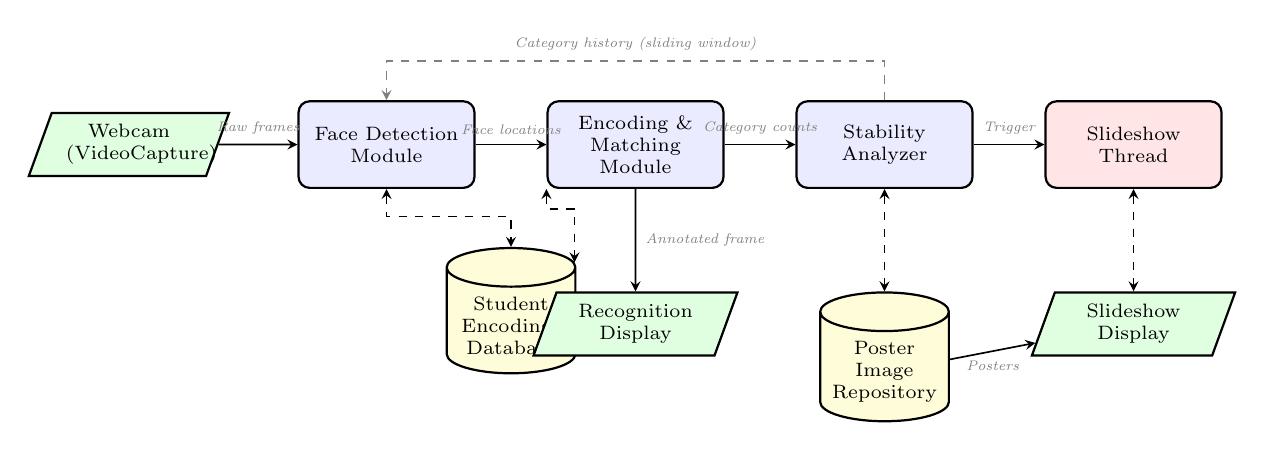
\begin{tikzpicture}[
    node distance=0.8cm and 0.8cm,
    module/.style={rectangle, rounded corners, draw=black, thick, fill=blue!8, minimum width=2.2cm, minimum height=1.1cm, text centered, text width=2.0cm, font=\scriptsize},
    store/.style={cylinder, draw=black, thick, fill=yellow!15, shape border rotate=90, minimum width=1.6cm, minimum height=1.0cm, text centered, text width=1.4cm, font=\scriptsize, aspect=0.3},
    io/.style={trapezium, trapezium left angle=70, trapezium right angle=110, draw=black, thick, fill=green!12, minimum width=1.8cm, minimum height=0.8cm, text centered, text width=1.6cm, font=\scriptsize},
    arrow/.style={->, >=stealth, semithick},
    darrow/.style={<->, >=stealth, semithick, dashed},
    lbl/.style={font=\tiny\itshape, text=gray}
]

% Row 1: Main processing pipeline (left to right)
\node[io] (cam) {Webcam\\(VideoCapture)};
\node[module, right=1.0cm of cam] (detect) {Face Detection\\Module};
\node[module, right=0.9cm of detect] (encode) {Encoding \&\\Matching Module};
\node[module, right=0.9cm of encode] (stab) {Stability\\Analyzer};
\node[module, right=0.9cm of stab, fill=red!10] (thread) {Slideshow\\Thread};

% Row 2: Data stores and output windows
\node[store, below=1.3cm of $(detect)!0.5!(encode)$] (studb) {Student\\Encodings\\Database};
\node[io, below=1.3cm of encode] (recwin) {Recognition\\Display};
\node[store, below=1.3cm of stab] (posterdb) {Poster Image\\Repository};
\node[io, below=1.3cm of thread] (slidewin) {Slideshow\\Display};

% Main pipeline arrows
\draw[arrow] (cam) -- node[above, lbl] {Raw frames} (detect);
\draw[arrow] (detect) -- node[above, lbl] {Face locations} (encode);
\draw[arrow] (encode) -- node[above, lbl] {Category counts} (stab);
\draw[arrow] (stab) -- node[above, lbl] {Trigger} (thread);

% Data store connections
\draw[darrow] (detect.south) -- ++(0,-0.35) -| (studb.north);
\draw[darrow] (encode.south west) -- ++(0,-0.25) -| (studb.north east);
\draw[darrow] (thread.south) -- node[right, lbl] {} (slidewin.north);
\draw[darrow] (stab.south) -- ++(0,-0.35) -| (posterdb.north);

% Output connections
\draw[arrow] (encode) -- node[right, lbl] {Annotated frame} (recwin);
\draw[arrow] (posterdb) -- node[below, lbl] {Posters} (slidewin);

% Feedback loop (stability -> detection)
\draw[arrow, dashed, gray] (stab.north) -- ++(0, 0.5) -| node[above, pos=0.25, lbl] {Category history (sliding window)} (detect.north);

\end{tikzpicture}
\caption{System architecture of the \textit{SlideSense} prototype. The main loop processes frames through detection, encoding, and stability analysis, while a separate daemon thread manages the slideshow display. Dashed arrows indicate data lookups; solid arrows indicate data flow.}
\label{fig:architecture}
\end{figure*}

\begin{itemize}
    \item \textbf{Face Detection Module:} Captures video frames from the webcam and identifies face regions using a Histogram of Oriented Gradients (HOG) based detector. To improve throughput, frames are downscaled to 25\% of their original resolution before detection.
    \item \textbf{Encoding \& Matching Module:} Computes a 128-dimensional face embedding for each detected face and compares it against pre-loaded student encodings using Euclidean distance. A match is accepted only when the distance falls below a threshold of 0.6, and a confidence score is derived as $C = \max\bigl(0,\;(1 - d) \times 100\bigr)$, where $d$ is the face distance.
    \item \textbf{Stability Analyzer:} Maintains a sliding window of the last 15 majority-category results. A category-specific slideshow is triggered only when a single category accounts for at least 10 of the 15 most recent observations, ensuring that transient misdetections do not cause erratic content switching.
    \item \textbf{Slideshow Display Thread:} Runs as a daemon thread, cycling through poster images for the identified category at a 3-second interval. The thread is terminated and replaced when the stable majority shifts to a different category.
\end{itemize}

\subsection{Data Organization}
The prototype organizes its data into two parallel directory hierarchies, each partitioned by academic stream (Science, Arts, Commerce):
\begin{itemize}
    \item \texttt{students/\{category\}/} -- Contains reference face images used to generate 128-dimensional encodings at startup. Each image corresponds to a single enrolled student.
    \item \texttt{posters/\{category\}/} -- Contains the informational poster images displayed during the category-specific slideshow.
\end{itemize}
During initialization, the system iterates over each category directory, loads all images, extracts face encodings using \texttt{dlib}'s ResNet-based metric learning model, and stores them in an in-memory dictionary keyed by category. This pre-computation step ensures that the real-time recognition loop only needs to perform distance comparisons rather than costly re-encoding of reference images.

\subsection{Recognition Pipeline}
The complete recognition pipeline, from frame capture to slideshow activation, is formalized in Algorithm \ref{alg:recognition}. The algorithm highlights several key design decisions: the frame-skipping strategy for computational efficiency, the distance-based matching with confidence scoring, and the temporal stability requirement that prevents premature content switching.

\begin{algorithm}[htbp]
\caption{Real-Time Face Recognition and Content Triggering Pipeline}
\label{alg:recognition}
\begin{algorithmic}[1]
\renewcommand{\algorithmicrequire}{\textbf{Input:}}
\renewcommand{\algorithmicensure}{\textbf{Output:}}
\REQUIRE Webcam video stream; pre-computed student encodings $E_c$ for each category $c \in \{$Science, Arts, Commerce$\}$; poster sets $P_c$
\ENSURE Category-specific slideshow displayed on screen

\STATE Initialize $\textit{history} \leftarrow []$, $\textit{frameCount} \leftarrow 0$
\STATE $N \leftarrow 3$ \COMMENT{Process every $N$-th frame}
\STATE $\tau \leftarrow 0.6$ \COMMENT{Distance threshold}
\STATE $W \leftarrow 15$, $T \leftarrow 10$ \COMMENT{Window size, trigger threshold}

\WHILE{system is active}
    \STATE $\textit{frame} \leftarrow$ capture frame from webcam
    \STATE $\textit{frameCount} \leftarrow \textit{frameCount} + 1$

    \IF{$\textit{frameCount} \mod N \neq 0$}
        \STATE Display previous annotated frame
        \STATE \textbf{continue}
    \ENDIF

    \STATE $\textit{small} \leftarrow$ resize $\textit{frame}$ to $0.25\times$
    \STATE $\textit{faces} \leftarrow$ detect face locations in $\textit{small}$
    \STATE $\textit{encodings} \leftarrow$ compute embeddings for $\textit{faces}$
    \STATE Initialize $\textit{count}_c \leftarrow 0$ for each category $c$

    \FORALL{face encoding $f$ in $\textit{encodings}$}
        \STATE $c^*, d^* \leftarrow \arg\min_{c} \min_{e \in E_c} \|f - e\|$
        \IF{$d^* < \tau$}
            \STATE $\textit{count}_{c^*} \leftarrow \textit{count}_{c^*} + 1$
            \STATE Annotate frame with $c^*$ and confidence $(1 - d^*) \times 100$
        \ELSE
            \STATE Label face as ``Unknown''
        \ENDIF
    \ENDFOR

    \STATE $m \leftarrow \arg\max_c \textit{count}_c$ \COMMENT{Majority category}
    \IF{$\sum_c \textit{count}_c > 0$}
        \STATE Append $m$ to $\textit{history}$
        \IF{$|\textit{history}| > W$}
            \STATE Remove oldest entry from $\textit{history}$
        \ENDIF
    \ENDIF

    \IF{mode$(history) = c_s$ \AND count$(c_s, history) \geq T$}
        \IF{$c_s \neq$ current slideshow category}
            \STATE Stop existing slideshow thread
            \STATE Launch new slideshow thread for $P_{c_s}$
            \STATE Reset $\textit{history}$
        \ENDIF
    \ENDIF
\ENDWHILE
\end{algorithmic}
\end{algorithm}

\subsection{Performance Optimization Strategies}
Real-time face recognition is computationally intensive, particularly on resource-constrained edge devices representative of IoT billboard controllers. The prototype employs three complementary optimization strategies, summarized in Table \ref{tab:optimizations}, to maintain interactive frame rates without dedicated GPU hardware.

\begin{table}[htbp]
\caption{Performance Optimization Strategies Employed in the Prototype}
\begin{center}
\begin{tabular}{p{2cm} p{2.5cm} p{3cm}}
\toprule
\textbf{Strategy} & \textbf{Implementation} & \textbf{Rationale} \\
\midrule
\textbf{Spatial Down-sampling} & Resize to $0.25\times$ before detection & Reduces pixel count by $16\times$, proportionally decreasing HOG computation time \\
\midrule
\textbf{Temporal Sub-sampling} & Process every 3\textsuperscript{rd} frame & Amortizes the cost of face encoding over multiple frames while maintaining visual responsiveness \\
\midrule
\textbf{Sliding-Window Stability} & Require $\geq$10/15 consistent results & Absorbs transient errors and prevents unnecessary slideshow restarts, reducing thread overhead \\
\bottomrule
\end{tabular}
\label{tab:optimizations}
\end{center}
\end{table}

The spatial down-sampling reduces the input resolution from the native camera resolution (typically $640 \times 480$) to $160 \times 120$ pixels for the detection pass. While face locations are subsequently scaled back to original coordinates for display annotation, matching is performed on the reduced representation. Temporal sub-sampling ensures that computationally expensive encoding operations occur only on every third frame, while intermediate frames reuse the most recent recognition result, maintaining a fluid user experience.

\subsection{Confidence Scoring and Visual Feedback}
The prototype provides real-time visual feedback through color-coded bounding boxes and per-face confidence labels, as illustrated conceptually in Fig. \ref{fig:visual_feedback}. Each recognized face is annotated with its matched academic category and a confidence percentage. The color scheme---green for Science, red for Arts, and blue for Commerce---provides an immediate visual indication of audience composition. Unrecognized faces are outlined in gray and labeled ``Unknown.''

\begin{figure}[htbp]
\centering
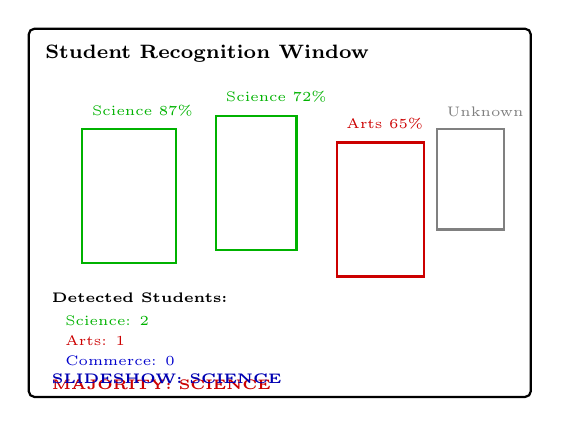
\begin{tikzpicture}[scale=0.85]
    % Simulated camera frame
    \draw[thick, rounded corners=2pt] (0,0) rectangle (7.5,5.5);
    \node[font=\scriptsize, anchor=north west] at (0.1, 5.4) {\textbf{Student Recognition Window}};

    % Face 1 - Science (green)
    \draw[green!70!black, thick] (0.8, 2.0) rectangle (2.2, 4.0);
    \node[font=\tiny, green!70!black, anchor=south west] at (0.8, 4.05) {Science 87\%};

    % Face 2 - Science (green)
    \draw[green!70!black, thick] (2.8, 2.2) rectangle (4.0, 4.2);
    \node[font=\tiny, green!70!black, anchor=south west] at (2.8, 4.25) {Science 72\%};

    % Face 3 - Arts (red)
    \draw[red!80!black, thick] (4.6, 1.8) rectangle (5.9, 3.8);
    \node[font=\tiny, red!80!black, anchor=south west] at (4.6, 3.85) {Arts 65\%};

    % Face 4 - Unknown (gray)
    \draw[gray, thick] (6.1, 2.5) rectangle (7.1, 4.0);
    \node[font=\tiny, gray, anchor=south west] at (6.1, 4.05) {Unknown};

    % HUD overlay - counts
    \node[font=\tiny, anchor=north west] at (0.2, 1.7) {\textbf{Detected Students:}};
    \node[font=\tiny, green!70!black, anchor=north west] at (0.4, 1.35) {Science: 2};
    \node[font=\tiny, red!80!black, anchor=north west] at (0.4, 1.05) {Arts: 1};
    \node[font=\tiny, blue!80!black, anchor=north west] at (0.4, 0.75) {Commerce: 0};
    \node[font=\tiny\bfseries, red!80!black, anchor=north west] at (0.2, 0.4) {MAJORITY: SCIENCE};

    % Slideshow indicator
    \node[font=\tiny\bfseries, blue!70!black, anchor=south west] at (0.2, 0.05) {SLIDESHOW: SCIENCE};
\end{tikzpicture}
\caption{Conceptual illustration of the recognition display window. Bounding boxes are color-coded by category (green = Science, red = Arts, blue = Commerce, gray = Unknown). A heads-up display overlay shows real-time counts and the current majority determination.}
\label{fig:visual_feedback}
\end{figure}

An on-screen heads-up display (HUD) continuously shows the per-category count of recognized students and highlights the current majority category. When a slideshow is active, an additional indicator at the bottom of the frame confirms which category's content is being displayed.

\subsection{Stability Detection Mechanism}
A critical design challenge is preventing the system from switching content erratically due to momentary misdetections or transient changes in the audience. The prototype addresses this through a temporal stability mechanism, depicted in Fig. \ref{fig:stability}.

\begin{figure}[htbp]
\centering
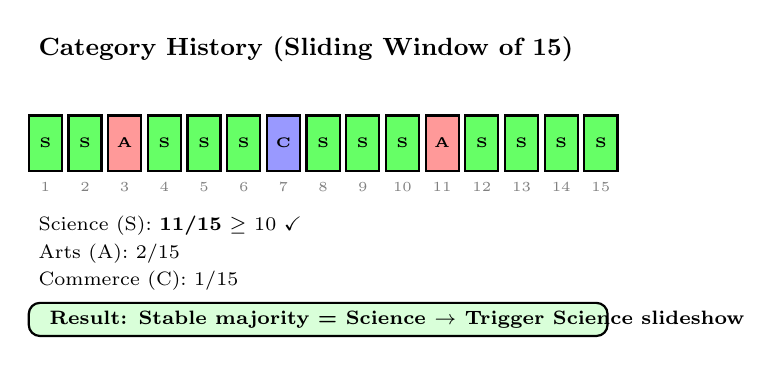
\begin{tikzpicture}[scale=0.7]
    % Title
    \node[font=\small\bfseries, anchor=west] at (0, 5.2) {Category History (Sliding Window of 15)};

    % Draw 15 boxes representing frames
    \foreach \i/\cat/\col in {
        1/S/green!60, 2/S/green!60, 3/A/red!40, 4/S/green!60, 5/S/green!60,
        6/S/green!60, 7/C/blue!40, 8/S/green!60, 9/S/green!60, 10/S/green!60,
        11/A/red!40, 12/S/green!60, 13/S/green!60, 14/S/green!60, 15/S/green!60
    } {
        \pgfmathsetmacro{\x}{(\i-1)*0.72}
        \draw[thick, fill=\col] (\x, 3.0) rectangle (\x+0.6, 4.0);
        \node[font=\tiny\bfseries] at (\x+0.3, 3.5) {\cat};
        \node[font=\tiny, gray] at (\x+0.3, 2.7) {\i};
    }

    % Tally
    \node[font=\scriptsize, anchor=west] at (0, 2.0) {Science (S): \textbf{11/15} $\geq$ 10 $\checkmark$};
    \node[font=\scriptsize, anchor=west] at (0, 1.5) {Arts (A): 2/15};
    \node[font=\scriptsize, anchor=west] at (0, 1.0) {Commerce (C): 1/15};

    % Result
    \draw[thick, rounded corners, fill=green!15] (0, 0.0) rectangle (10.5, 0.6);
    \node[font=\scriptsize\bfseries, anchor=west] at (0.2, 0.3) {Result: Stable majority = Science $\rightarrow$ Trigger Science slideshow};
\end{tikzpicture}
\caption{Illustration of the sliding-window stability mechanism. Each cell represents one processed frame's majority category. A slideshow is triggered only when a single category accounts for $\geq$10 of the 15 most recent observations (here, Science with 11/15).}
\label{fig:stability}
\end{figure}

The system maintains a first-in, first-out (FIFO) queue of the last 15 processed frames' majority categories. After each recognition cycle, the mode of this window is computed. A slideshow transition occurs only when:
\begin{enumerate}
    \item A single category reaches the threshold of $\geq$10 occurrences within the window, \textit{and}
    \item That category differs from the currently active slideshow.
\end{enumerate}
Upon triggering, the history buffer is cleared to prevent stale data from prematurely re-triggering a transition. This approach provides a configurable trade-off between responsiveness and stability---a larger window or higher threshold yields more stable behavior at the cost of slower reaction to genuine audience changes.

\subsection{Slideshow Content Delivery}
When a stable majority is confirmed, the system spawns a daemon thread that creates a dedicated display window (800$\times$600 pixels) and cycles through the poster images associated with the identified category. Each poster is displayed for 3 seconds, with a title overlay indicating the active category and the current slide number. The thread monitors a shared \texttt{stop\_slideshow} flag, allowing the main recognition loop to gracefully terminate it when the audience composition shifts. This decoupled architecture ensures that the slideshow display does not block the recognition pipeline, maintaining continuous real-time monitoring.

% ====================================================================

\section{Applications}
The proposed smart billboard system has several applications designed to improve campus communication and efficiency \cite{D1}:
\begin{itemize}
    \item \textbf{Department-Specific Updates:} Displaying departmental news, announcements, and event notifications targeted to the relevant student groups \cite{D1, D0}.
    \item \textbf{Timetable and Schedule Changes:} Announcing timetable changes, registration deadlines, or workshop opportunities to specific cohorts of students \cite{D1}.
    \item \textbf{Emergency Alerts:} In case of an emergency, the billboards can be used to broadcast campus-wide safety alerts instantly \cite{D1}.
    \item \textbf{Enhanced Student Engagement:} By providing timely and relevant information, the system aims to boost student engagement and reduce reliance on physical notices \cite{D1, D0}.
\end{itemize}

\section{Feasibility and Ethical Considerations}
While the proposed system offers numerous benefits in theory, its practical implementation hinges on overcoming significant and deeply intertwined technical and ethical hurdles. A thorough feasibility analysis---now informed by hands-on experience with the \textit{SlideSense} prototype---reveals profound challenges that question the viability of the project as currently conceived, particularly concerning the reliance on student ID photos as a primary data source. These technical limitations are not merely operational inconveniences; they directly feed into the ethical landscape, creating a system that risks being not only ineffective but also inequitable and invasive.

The core technical challenge lies in the vast gap between recognition in controlled environments versus ``in-the-wild'' scenarios like a dynamic university campus \cite{R41}. While algorithms can achieve near-perfect accuracy (up to 99.97\%) when matching high-quality, posed photographs, this performance degrades dramatically in real-world conditions \cite{R41, R80}. The project's target accuracy of 85\% appears highly optimistic, as research shows error rates can climb from 0.1\% in ideal settings to over 9\% when matching against images captured in uncontrolled environments \cite{R41}. This is due to a confluence of factors: poor or variable lighting, suboptimal camera angles, and partial facial occlusions from hats or other people are common on a campus and are not effectively compensated for by current algorithms \cite{R65}. Perhaps most critically, the natural aging of students over their academic tenure means that a photo taken in their first year may be a poor reference for identification three or four years later, a factor known to increase error rates significantly \cite{R41, R74}. These factors critically impact the system's accuracy, making it unlikely to reliably perform its primary function.

The prototype's development experience corroborated these concerns. Even with spatial down-sampling to $0.25\times$ and temporal sub-sampling (processing every 3\textsuperscript{rd} frame), the system required careful environmental control to achieve acceptable recognition rates. The reliance on a single reference image per student---a realistic constraint mirroring the ID-photo scenario---proved particularly limiting, as it offered no ``within-person variability'' to account for changes in pose, expression, or appearance. The stability mechanism (requiring 10/15 consistent frames) was introduced precisely because individual frame-level recognition was too unreliable to drive content decisions directly.

Table \ref{tab:feasibility} provides a scorecard summarizing these challenges, and Table \ref{tab:proto_params} maps the prototype's concrete parameter choices to these feasibility factors.

\begin{table}[htbp]
\caption{Prototype Configuration Parameters and Their Feasibility Implications}
\begin{center}
\begin{tabular}{p{2.2cm} p{1.3cm} p{4cm}}
\toprule
\textbf{Parameter} & \textbf{Value} & \textbf{Implication} \\
\midrule
Distance threshold & 0.6 & Balances false positives vs.\ false negatives; stricter values reject more true matches \\
\midrule
Frame resize & $0.25\times$ & Necessary for real-time speed but reduces facial detail available for matching \\
\midrule
Frame skip & Every 3\textsuperscript{rd} & Trades detection continuity for CPU feasibility on edge hardware \\
\midrule
Stability window & 15 frames & Absorbs noise but introduces 1--2 second latency before content switch \\
\midrule
Trigger threshold & 10/15 & High bar prevents false triggers but may miss brief audience changes \\
\midrule
Slide interval & 3 sec & Fixed rotation; no adaptation to audience dwell time \\
\bottomrule
\end{tabular}
\label{tab:proto_params}
\end{center}
\end{table}

Furthermore, the deployment of FRT on campus forces a confrontation with a complex ethical and legal landscape. The system's operation---passively identifying students without their active consent---is in direct tension with data privacy principles. In the United States, the Family Educational Rights and Privacy Act (FERPA) classifies ``facial characteristics'' as a biometric record, which is a form of Personally Identifiable Information (PII) \cite{R64, R67}. The collection and use of such data without explicit, opt-in consent is legally precarious and risks transforming the campus into an environment of pervasive surveillance, which can create a chilling effect on free expression and association \cite{R30, R47}.

Beyond privacy, the issue of algorithmic bias presents a fundamental challenge to fairness and equity. It is well-documented that leading FRT algorithms perform less accurately for women and people of color, with some studies showing misidentification rates 10 to 100 times higher for Black or East Asian faces than for white faces \cite{R22}. This is largely due to non-diverse training datasets \cite{R34}. Deploying such a system would institutionalize a form of digital discrimination, where the technology works better for some students than others, directly undermining the university's commitment to inclusion. Therefore, a robust ethical framework must be a non-negotiable prerequisite for any implementation. Best practices for transparency, informed consent, bias mitigation, and stringent data security must be established and rigorously enforced \cite{R17, R9}. Table \ref{tab:ethics} outlines a checklist for such an ethical implementation, drawing on established principles for data protection and accountability.

\begin{table*}[htbp]
\caption{Feasibility Scorecard for ID Photo-Based Recognition}
\begin{center}
\begin{tabular}{p{3cm} p{5cm} p{2cm} p{6cm}}
\toprule
\textbf{Feasibility Factor} & \textbf{Challenge Description} & \textbf{Impact on Accuracy} & \textbf{Potential Mitigation (and Associated Costs/Risks)} \\
\midrule
\textbf{Source Image Quality} & Student ID photos are static, single-instance images taken under variable conditions, lacking the ``within-person variability'' needed for robust model training. & High & Re-capture multiple high-quality, varied images of each student. (High logistical cost, increased data storage, significant privacy implications). \\
\textbf{Environmental Variation} & Uncontrolled and changing lighting, shadows, and weather conditions in campus locations degrade image quality for live capture. & High & Install high-end cameras with superior low-light performance and dynamic range; supplement with controlled lighting. (High hardware cost). \\
\textbf{Pose and Occlusion} & Students will be in motion, at various angles to the camera, and partially obscured by accessories (hats, glasses) or other people. & High & Utilize advanced 3D recognition algorithms or multi-camera systems to capture faces from multiple angles. (Increased software complexity and hardware cost). \\
\textbf{Student Aging} & A student's appearance can change significantly over their 1--4 year tenure, creating a mismatch with their initial ID photo. & High & Mandate annual photo recapture for all students to update the database. (High logistical and administrative cost, student inconvenience, privacy concerns). \\
\bottomrule
\end{tabular}
\label{tab:feasibility}
\end{center}
\end{table*}

\begin{table*}[htbp]
\caption{Checklist of Best Practices for Ethical Implementation}
\begin{center}
\begin{tabular}{p{3cm} p{6cm} p{7cm}}
\toprule
\textbf{Best Practice} & \textbf{Implementation Action} & \textbf{Supporting Rationale} \\
\midrule
\textbf{Transparency} & Publish a clear, accessible policy detailing the system's purpose, data handling procedures, and limitations. Mandate physical signage at all locations where FRT is active. & Public and private entities should be required to disclose when and how facial recognition is used, what data is collected, and why \cite{R36, R31}. \\
\textbf{Informed Consent} & Implement a mandatory, explicit opt-in system before collecting or using any student's biometric data for non-essential services. Ensure consent is freely given and can be revoked. & The power imbalance in a school setting makes true consent difficult; an opt-in model is the only way to ensure voluntary participation \cite{R11}. \\
\textbf{Bias Mitigation} & Use diverse datasets for training and conduct regular, independent audits to test for and report on accuracy disparities across demographic groups. & FRT algorithms are known to perform less accurately for women and people of color. Audits are essential to identify and address this systemic harm \cite{R36, R12}. \\
\textbf{Data Security} & Employ end-to-end encryption for all biometric data. Implement strict access controls and a clear data retention and deletion schedule. & Biometric data is unchangeable if breached. Strong security is essential to protect against theft and misuse \cite{R8, R36}. \\
\textbf{Purpose Limitation} & Strictly prohibit the use of collected data for any purpose beyond the single, approved application (e.g., billboard content). Ban use for disciplinary or law enforcement purposes. & This prevents ``function creep,'' where data collected for one purpose is later repurposed for more invasive surveillance without new consent \cite{R9, R3}. \\
\textbf{Accountability} & Establish an independent oversight committee with student, faculty, and administrative representation to approve and monitor all FRT deployments. & An appropriate level of human control and oversight is necessary for uses that may affect people in meaningful ways \cite{R31}. \\
\bottomrule
\end{tabular}
\label{tab:ethics}
\end{center}
\end{table*}

\newpage
\section{Observations from Prototype Development}
The development and testing of the \textit{SlideSense} prototype yielded several observations that are instructive for the broader feasibility discussion:

\begin{enumerate}
    \item \textbf{Single-image enrollment is fragile.} The prototype's student database contained only one reference image per student per category---a constraint that mirrors the ID-photo scenario described in the feasibility analysis. In practice, this yielded highly variable confidence scores depending on the subject's pose, lighting, and distance from the camera, confirming that ``within-person variability'' in training data is essential for robust recognition \cite{R41}.

    \item \textbf{Computational cost necessitates trade-offs.} Even on a modern desktop CPU, real-time face encoding at full resolution was infeasible. The combination of $0.25\times$ spatial down-sampling and 3-frame temporal sub-sampling was necessary to maintain interactive frame rates, but each optimization introduces its own accuracy penalty: reduced spatial detail and the possibility of missing faces that appear briefly between processed frames.

    \item \textbf{Stability buffering masks individual-frame unreliability.} The 10/15-frame stability requirement was not a design choice driven by user experience alone; it was an engineering necessity to compensate for the high variance in per-frame recognition results. This observation directly supports the literature's claim that FRT accuracy in uncontrolled settings is substantially lower than laboratory benchmarks \cite{R17, R41}.

    \item \textbf{The system determines group composition, not individual identity.} A notable design distinction is that the billboard system requires only the \textit{majority category} of the audience, not the identity of any individual student. This ``group-level'' approach is less privacy-invasive than individual identification but still requires processing each student's biometric data to arrive at the aggregate result, meaning the privacy concerns remain substantively unchanged.
\end{enumerate}

\newpage
\section{Conclusion}
This paper has introduced a framework for a smart digital billboard system aimed at making campus communication more personal and effective, and has supplemented the theoretical analysis with empirical evidence from a functional prototype. The development of \textit{SlideSense} demonstrated that the core technical pipeline---from camera capture through face detection, encoding-based matching, stability analysis, and category-specific content delivery---is implementable with open-source tools. However, the prototype also made tangible the significant gap between controlled demonstrations and robust real-world deployment.

A critical evaluation of the proposed methodology reveals that while the vision is compelling, its foundation is technologically fragile and ethically fraught. The successful deployment of the proposed system is predicated on achieving an 85\% recognition accuracy, a target that both our literature analysis and prototype experience suggest is unworkable given the limitations of using a static ID photo database for real-time identification in a dynamic campus environment \cite{D1}. The significant drop in accuracy in ``in-the-wild'' settings, combined with challenges like environmental variability and student aging, indicates a high probability of system failure, negating its intended benefits of improved student engagement and administrative efficiency \cite{R17}. The prototype's reliance on aggressive down-sampling, frame skipping, and a high stability threshold (10/15 frames) underscores these limitations: each optimization was introduced not as an enhancement, but as a necessary concession to make an inherently unreliable process minimally functional.

More profoundly, this project forces a consideration of what kind of campus environment we aim to create. The shift from passive signage to active, automated surveillance is not a minor technological upgrade; it is a fundamental change in the relationship between the university and its students. The meager gains of displaying slightly more relevant information do not justify the immense risks of normalizing a surveillance culture, perpetuating algorithmic bias against marginalized communities, and navigating the precarious legal landscape of student data privacy under FERPA \cite{R18, R12, R30}.

Therefore, we conclude with a strong recommendation to reconsider this approach. The ultimate goal should not be merely to deploy novel technology, but to do so in a manner that is effective, equitable, and respectful of the community it serves. Future work should prioritize exploring privacy-preserving alternatives, such as opt-in, app-based systems or interactive QR codes, which can achieve personalization without resorting to mass surveillance \cite{R70}. Expanding to a full, campus-wide network should only be a long-term goal if and when the technology matures to a point where accuracy is guaranteed and the profound ethical concerns have been fully and transparently addressed through a robust governance framework. The path to a truly ``smart'' campus is paved not just with innovation, but with a steadfast commitment to the privacy, dignity, and well-being of every student.

\newpage
\begin{thebibliography}{00}

\bibitem{R1}
M. Bellaj, A. Bendahmane, A. Zbitou, and H. Gueddah, ``A systematic review of smart campus technologies to improve students' educational experiences,'' 2024. [Online]. Available: https://www.researchgate.net/publication/384653776 [1]

\bibitem{D1}
N. Luke, C. S, S. Yadav, S. V. S, and S. Saxena, ``A Smart Campus Framework for Personalized Information Delivery Using Intelligent Digital Billboards,'' 2024. [2]

\bibitem{D0}
N. Luke and C. S, ``Smart Campus Enhancing Student Life with AR/VR Digital Billboard for Christites,'' Presentation, Christ (Deemed to be University). [3]

\bibitem{R18}
M. Andrejevic and N. Selwyn, ``Facial recognition technology in schools: critical questions and concerns,'' \textit{Learning, Media and Technology}, vol. 45, no. 2, pp. 115-128, 2020. [4]

\bibitem{R9}
S. Parthasarathy, C. Galligan, H. Rosenfeld, and M. Kleinman, ``Cameras in the Classroom: Facial Recognition Technology in Schools,'' \textit{Science, Technology, and Public Policy Program, University of Michigan}, Ann Arbor, MI, Aug. 2020. [5, 6, 7, 8]

\bibitem{R4}
Z. Shao and Y. Li, ``Facial Recognition Technology: College Students' Perspectives in the US,'' \textit{Trends in Sociology}, vol. 2, no. 2, pp. 45-55, 2024. [9, 10]

\bibitem{R8}
T. Hertz and E. Adar, ``A First Look into Users' Perceptions of Facial Recognition in the Physical World,'' in \textit{Proc. 2021 CHI Conf. Human Factors in Computing Systems (CHI '21)}, 2021, pp. 1-14. [11]

\bibitem{R12}
``Why Racial Bias is Prevalent in Facial Recognition Technology,'' \textit{Harvard Journal of Law \& Technology}, Nov. 3, 2020. [Online]. Available: https://jolt.law.harvard.edu/digest/why-racial-bias-is-prevalent-in-facial-recognition-technology [12]

\bibitem{R16}
S. Yuan, et al., ``Impact of Face-Recognition-Based Access Control System on College Students' Sense of School Identity and Belonging During COVID-19 Pandemic,'' \textit{Frontiers in Psychology}, vol. 13, 2022. [13]

\bibitem{R3}
C. Garvie, A. M. Smith, and J. Frankle, ``Beyond surveillance: privacy, ethics, and regulations in face recognition technology,'' \textit{PMC}, 2024. [Online]. Available: https://pmc.ncbi.nlm.nih.gov/articles/PMC11256005/ [14]

\bibitem{R11}
``The problem with facial recognition in schools,'' \textit{9ine}, Jul. 30, 2024. [Online]. Available: https://www.9ine.com/newsblog/the-problem-with-facial-recognition-in-schools [15]

\bibitem{R31}
``6 guidelines for facial recognition to build trust,'' \textit{Thales Group}, Jun. 12, 2023. [Online]. Available: https://www.thalesgroup.com/en/markets/digital-identity-and-security/government/inspired/facial-recognition-regulation [16]

\bibitem{R36}
``Ethics of Facial Recognition: Key Issues and Solutions,'' \textit{G2 Learning Hub}, Jul. 25, 2025. [Online]. Available: https://learn.g2.com/ethics-of-facial-recognition [17]

\bibitem{R41}
P. Grother, G. Quinn, and M. Ngan, ``Face In Video Evaluation (FIVE) Face Recognition of Non-Cooperative Subjects,'' \textit{NIST Interagency Report 8173}, National Institute of Standards and Technology, Gaithersburg, MD, Apr. 2017. [18]

\bibitem{R64}
``Biometric Record,'' \textit{U.S. Department of Education}. [Online]. Available: https://studentprivacy.ed.gov/content/biometric-record. [Accessed: Oct. 7, 2025]. [19, 20]

\bibitem{R12_2}
O. T. T., O. F. T., and O. A. J., ``Development of an Attendance Management System Using Facial Recognition Technology,'' \textit{Journal of Engineering Research and Reports}, vol. 26, no. 10, pp. 297--307, 2024. [21]

\bibitem{R30}
N. Bala, ``The Danger of Facial Recognition in Our Children's Classrooms,'' \textit{Duke Law \& Technology Review}, vol. 18, pp. 248-269, 2020. [22, 23]

\bibitem{R17}
W. A. Carter, ``How accurate are facial recognition systems, and why does it matter?'' \textit{Center for Strategic and International Studies}, Apr. 14, 2020. [Online]. Available: https://www.csis.org/blogs/strategic-technologies-blog/how-accurate-are-facial-recognition-systems-and-why-does-it [24]

\bibitem{R11_2}
A. H. Ali, et al., ``Student attendance with face recognition (LBPH or CNN): Systematic literature review,'' \textit{Procedia Computer Science}, vol. 216, pp. 31-38, Jan. 2023. [25]

\bibitem{R22}
S. S. Kumar, et al., ``Automatic Attendance System, Using Face Detection and Machine Learning,'' \textit{International Journal of Novel Research and Development (IJNRD)}, vol. 9, no. 2, Feb. 2024. [26]

\end{thebibliography}

\end{document}
